\section{Results}
\label{sec:results}
We begin the results section by performing an error and convergence 
analysis of the constructed surrogate using the PC expansions to 
establish its validity in Section~\ref{sec:analysis}.  In Section
~\ref{sec:forward}, we present a statistical analysis to quantify the 
uncertainty in the predicted water surface elevation in addition to a 
sensitivity analysis that enables us to rank the impact of the 
different Manning's $n$ coefficients on the uncertainty. Finally, 
in Section~\ref{sec:inverse}, we present the results of the inverse problem 
where we determine the posterior distributions of the input uncertain
parameters and analyze them in light of the available gauge data.
\subsection{Error and convergence study}
\label{sec:analysis}

Figure~\ref{fig:rlzs} shows the evolution of the
water surface elevation for the 125 realizations obtained 
to compute the PC expansions at the four different gauge 
locations. We notice that the variation in surface elevation 
is negligible during the first hour at gauge number 21418 
and during the first two hours for the remaining gauges
as the plots of the different realizations are seen to superimpose.
However, a noticeable uncertainty in the surface 
elevation can be seen  at all gauges as indicated from the thickness 
of the bands formed by the plots of the realizations. This uncertainty
occurs till the end of the simulations.
\begin{figure}[h]
\centering
\begin{tabular}{clc}        
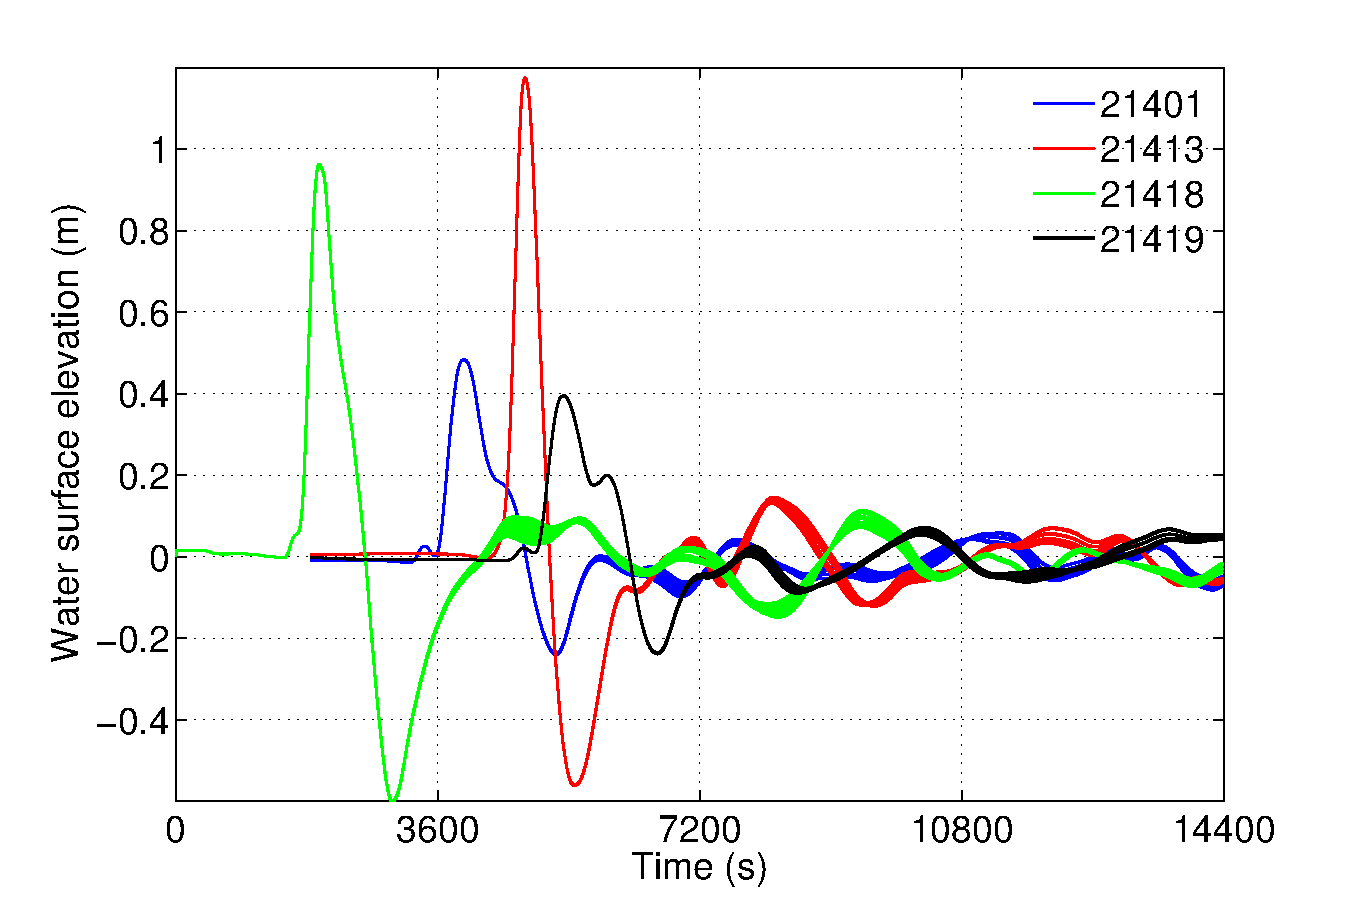
\includegraphics[width=0.6\textwidth]{figures/rlzs_gauges.pdf} 
\end{tabular}
\caption{125 Geoclaw realizations at different gauge locations.}
\label{fig:rlzs}
\end{figure}


In order to check the consistency of the approximation, we compare
 water surface elevation from the realizations 
with those obtained from the PC surrogate. The different curves
show an excellent agreement (not shown) for all times. We also define
an error metric that measures the relative normalized root mean-square error between the left hand side function 
in Equation~(\ref{eq:stochseries})
and its PC representation at the sampling points:
\begin{equation} 
   E = \frac{\displaystyle
         \left(\sum_{\xxi \in \NISP} \left|U(\xxi) - \sum_{k = 0}^{P}
U_k\Psi_k(\xxi)\right|^2
         \right)^{1/2}}
        {\displaystyle
          \left(\sum_{\xxi \in \NISP} \left|U(\xxi)\right|^2\right)^{1/2} 
          },
\label{eq:error}
\end{equation}
where $\NISP$ is the 125-member ensemble obtained using the PC algorithm. 
This error metric calculated at the different gauge locations is shown in Figure~\ref{fig:error};
the largest relative normalized error for 
water surface elevation is about 0.1\% . 
\begin{figure}[h]
\centering
\begin{tabular}{clc}        
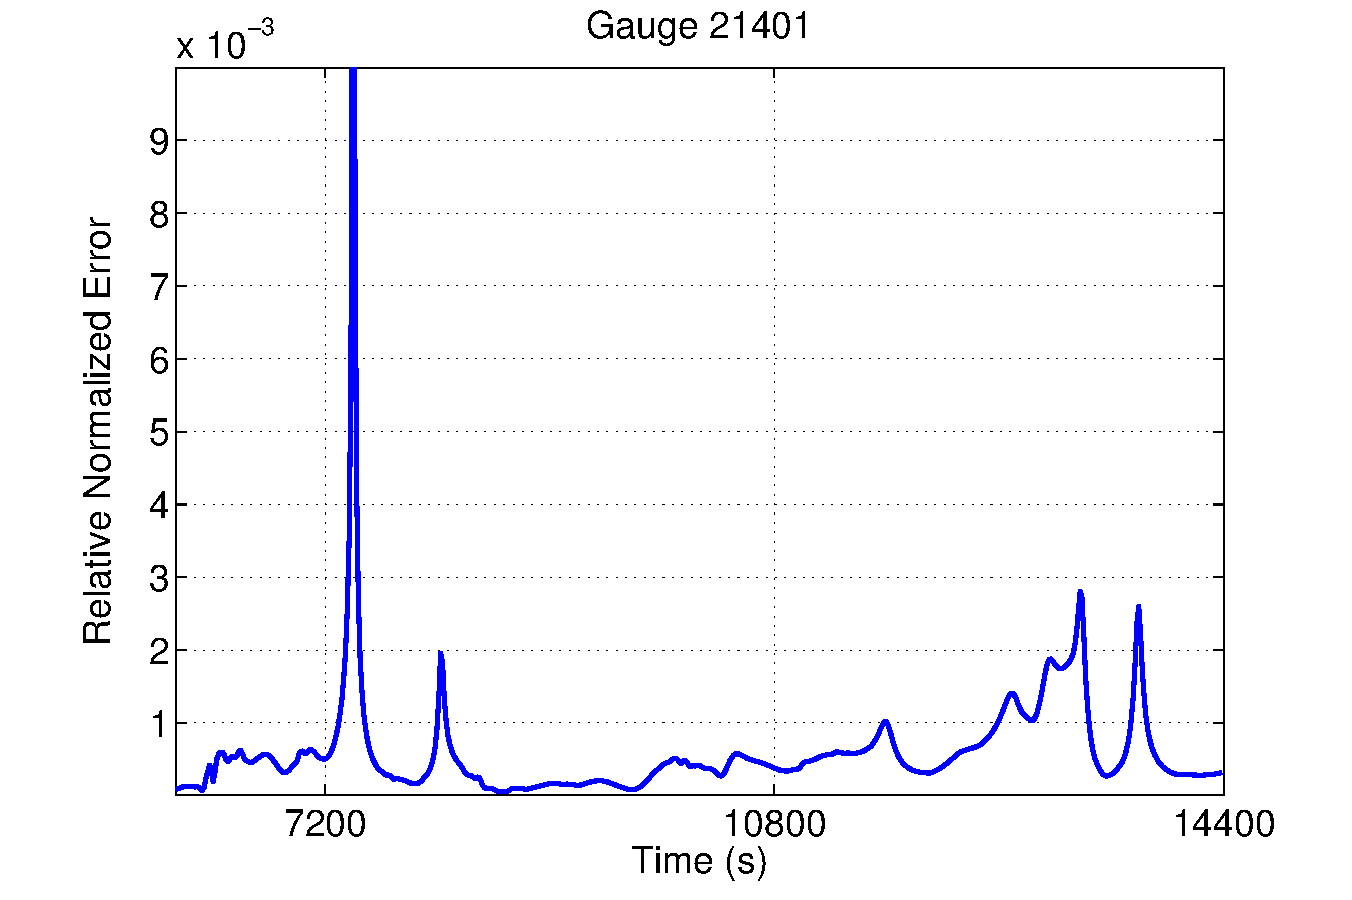
\includegraphics[width=0.5\textwidth]{figures/error_gauge1.pdf} &
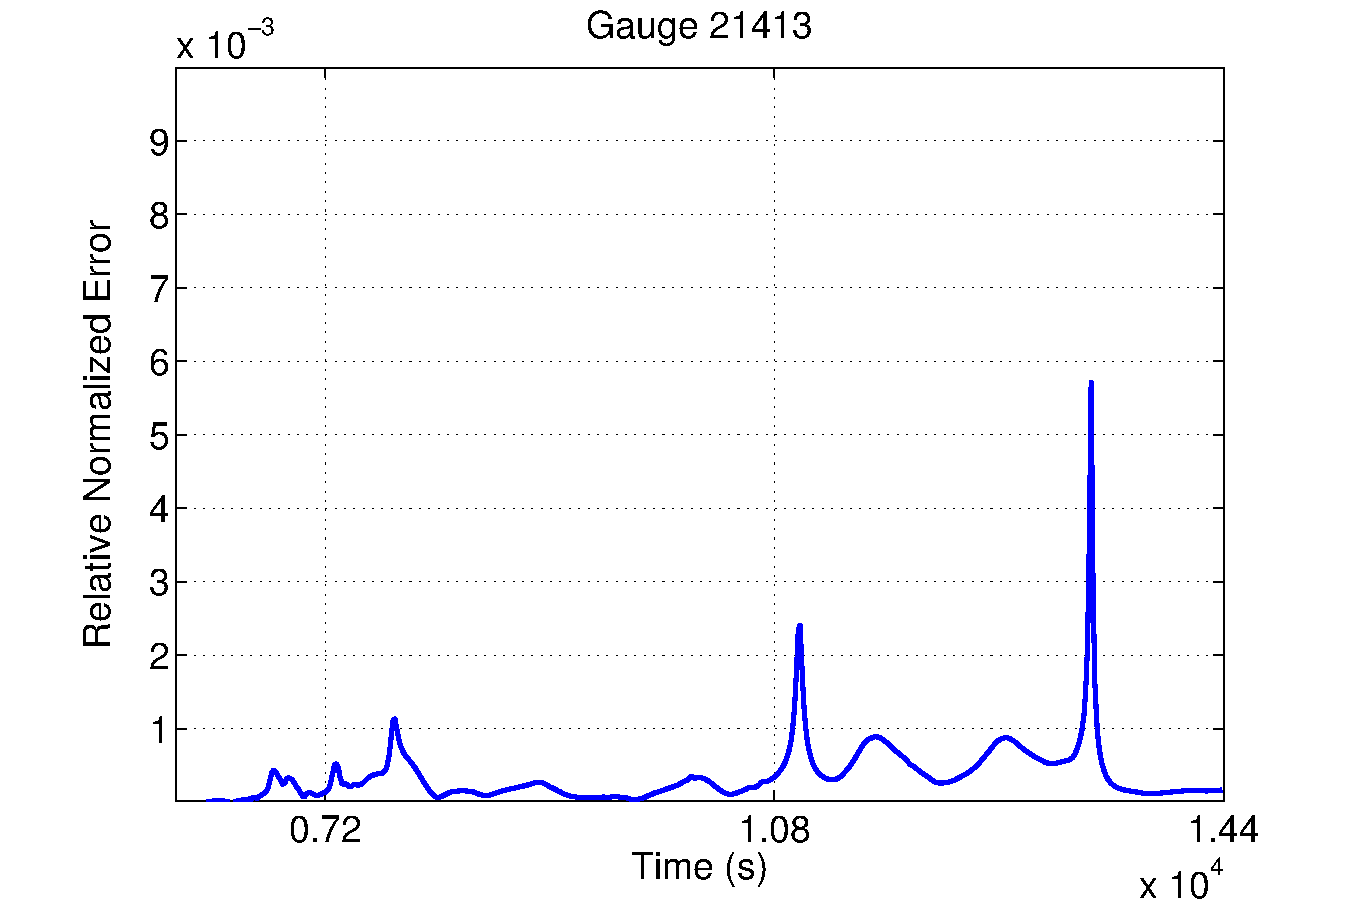
\includegraphics[width=0.5\textwidth]{figures/error_gauge2.pdf} \\
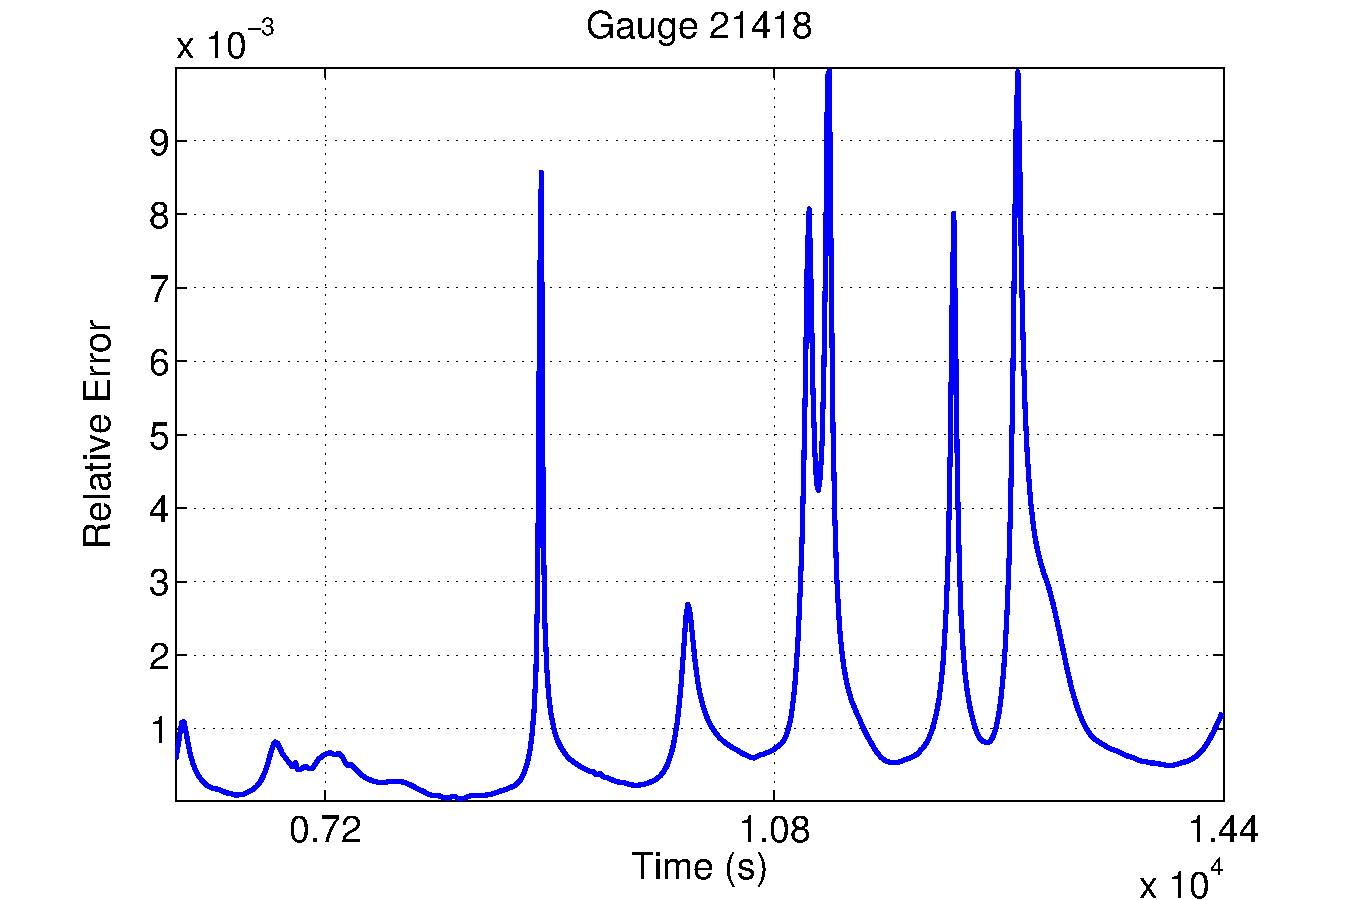
\includegraphics[width=0.5\textwidth]{figures/error_gauge3.pdf} &
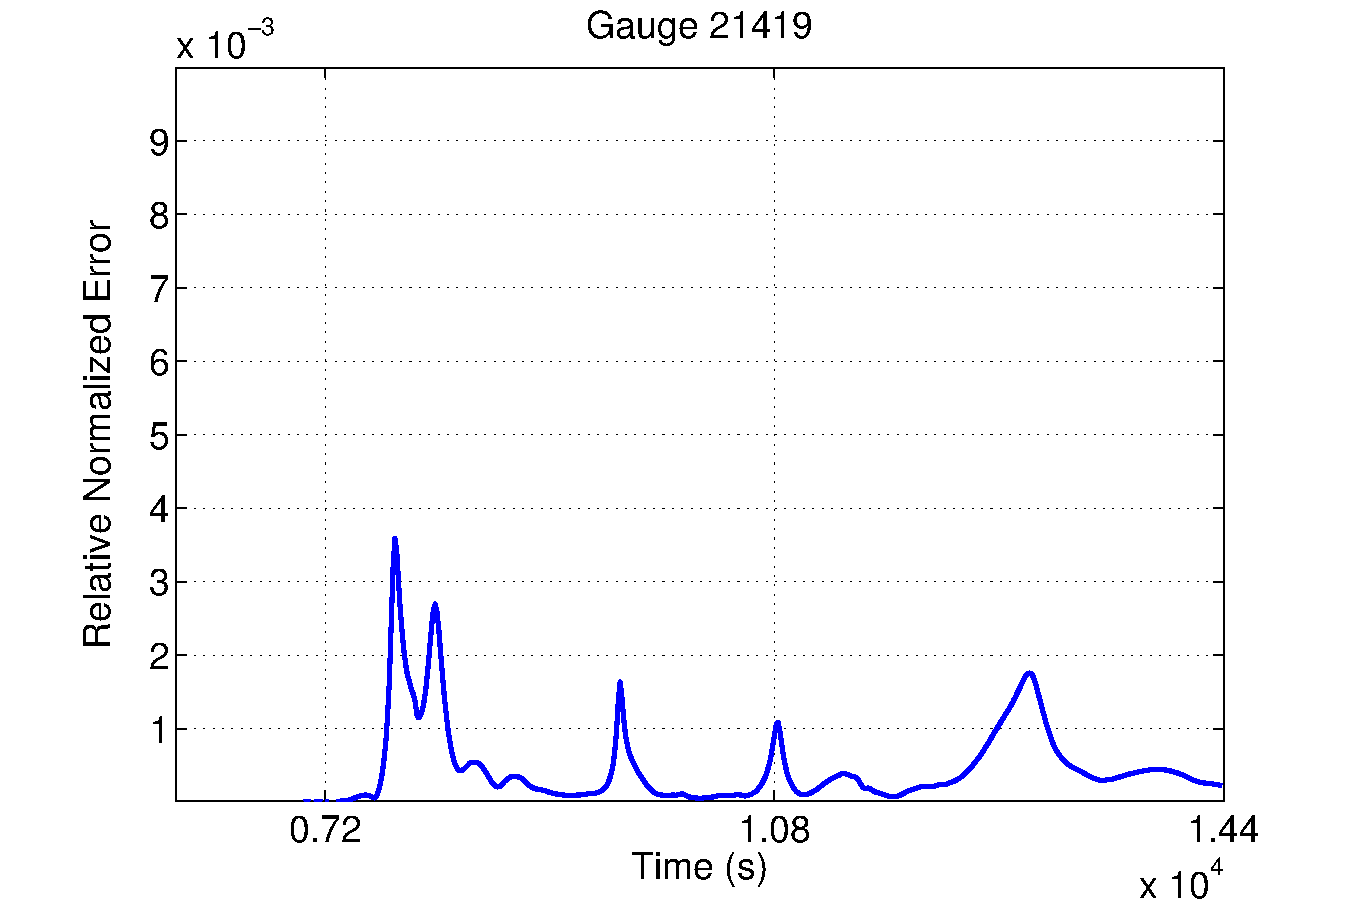
\includegraphics[width=0.5\textwidth]{figures/error_gauge4.pdf} 

\end{tabular}
\caption{125 Geoclaw realizations at different gauge locations.}
\label{fig:error}
\end{figure}

%Contour maps of the relative normalized error for the entire simulation region are 
%shown in Figure~\ref{fig:error2D} for various depths and dates to confirm the error trends of the
%analysis box.  The error is largest after the wind
%intensifies (bottom row) for all depths. For either day, the maximum
%error is located at 50~m which coincides with the depth of the
%original mixed layer measured by the AXBT. The maximum magnitude
%recorded is about 1\% and occurs on Sep~18. The
%elevated error region is located to the right of the storm and
%extends from the surface down to 50~m, after which the impact of the
%input uncertainty decreases substantially.  For the purpose of our
%current study, and given that the majority of AXBT data are at
%depth, the surrogate's errors are considered acceptable and small.

 
A final check consists of verifying whether the probability density
functions (pdfs) of water surface elevation at the different gauge locations
converges with increased order of the PC representation.  Sample
water surface elevation pdfs are shown in Figure~\ref{fig:pdfs2}
and Figure~\ref{fig:pdfs3}

\begin{figure}[h]
\centering

\begin{tabular}{clcl}
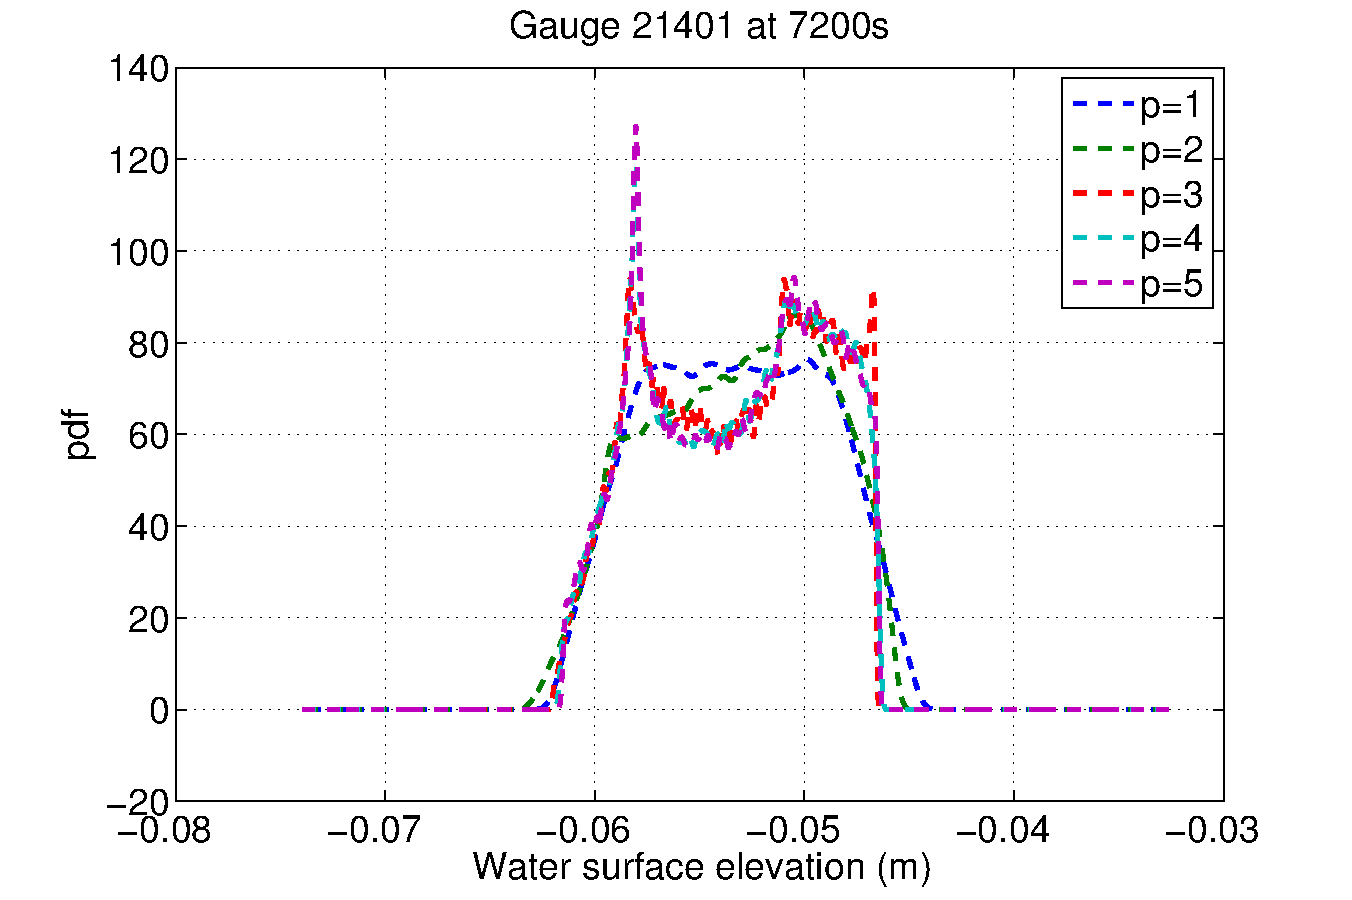
\includegraphics[width=0.5\textwidth]{figures/pdfs1_2.pdf} &
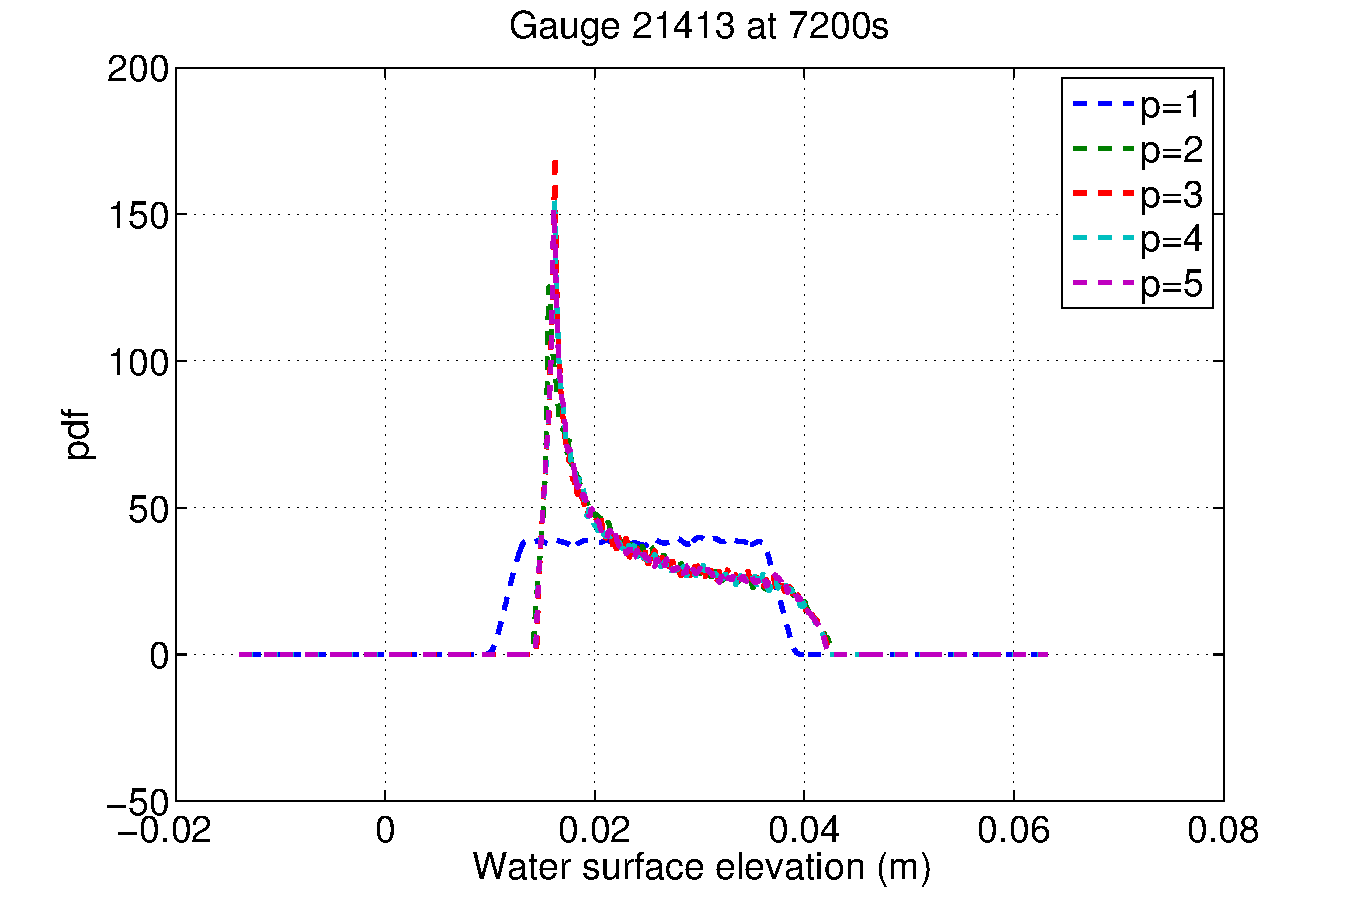
\includegraphics[width=0.5\textwidth]{figures/pdfs2_2.pdf} \\
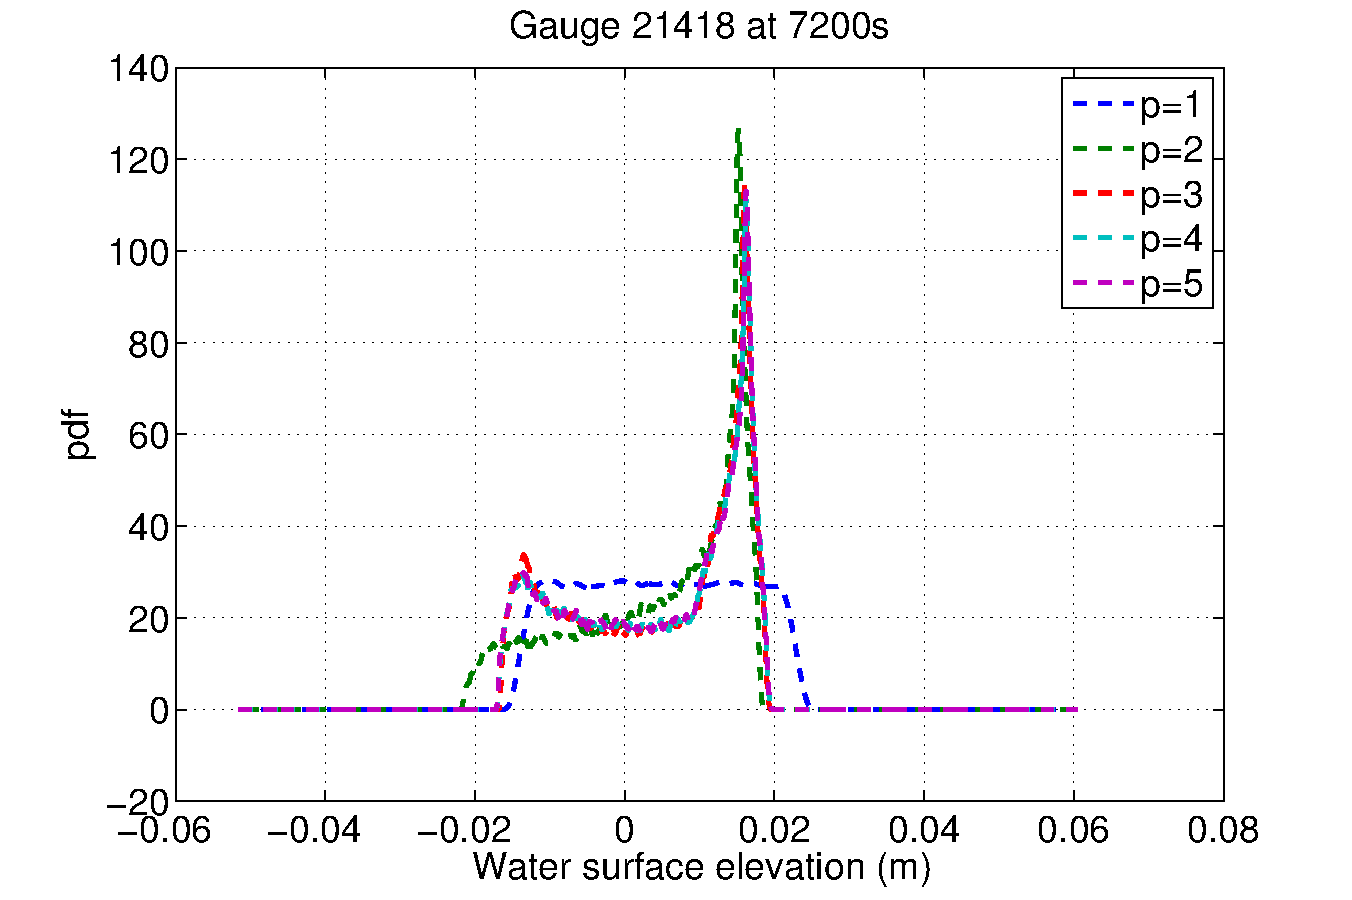
\includegraphics[width=0.5\textwidth]{figures/pdfs3_2.pdf} &
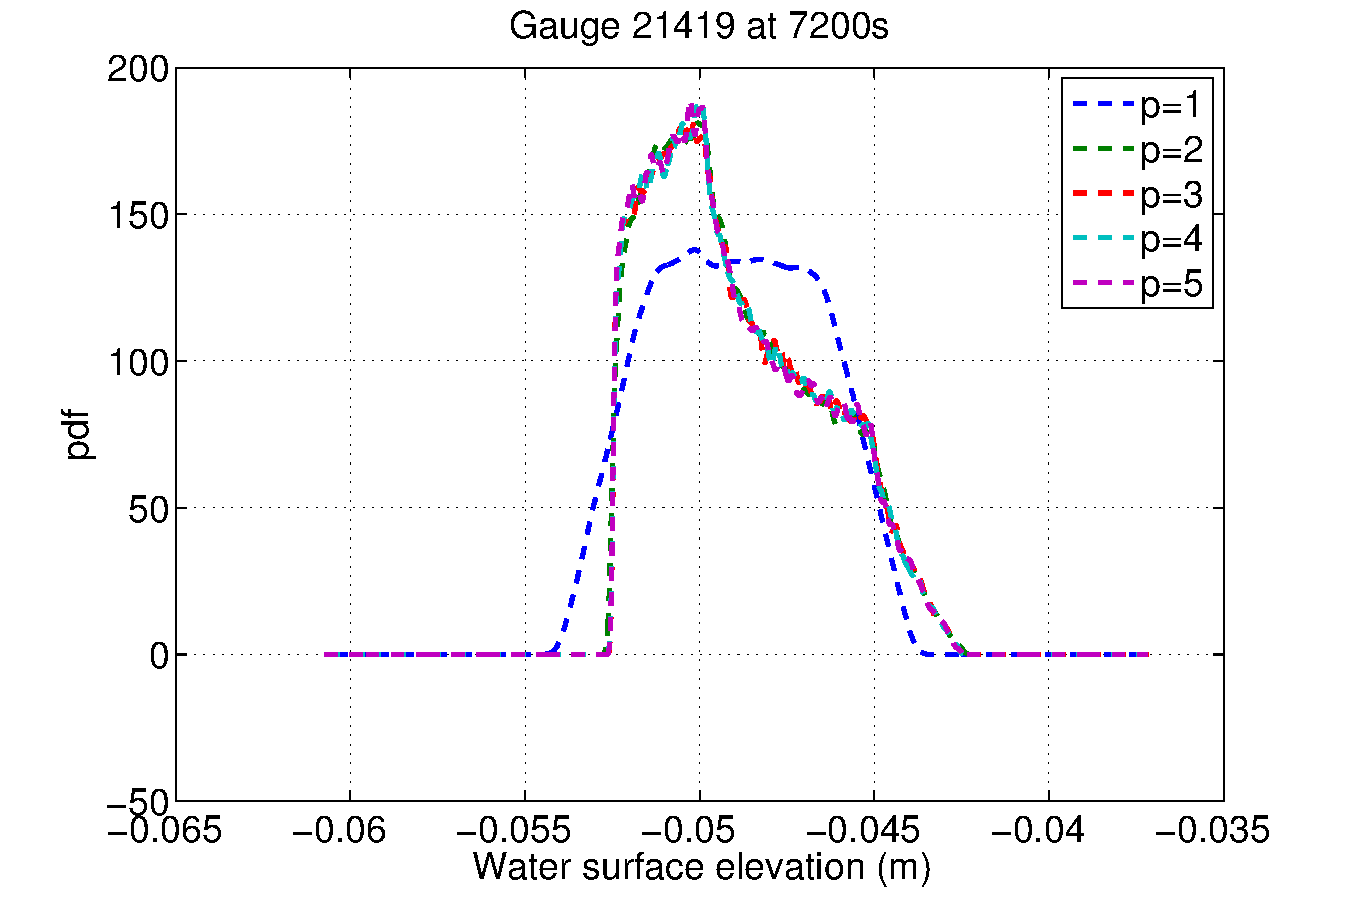
\includegraphics[width=0.5\textwidth]{figures/pdfs4_2.pdf}
\end{tabular}
\caption{pdf of water surface elevation at the different gauge locations at t = 7200 s.}
\label{fig:pdfs2}
\end{figure}
        
\begin{figure}[h]
\centering
\begin{tabular}{clc}
        
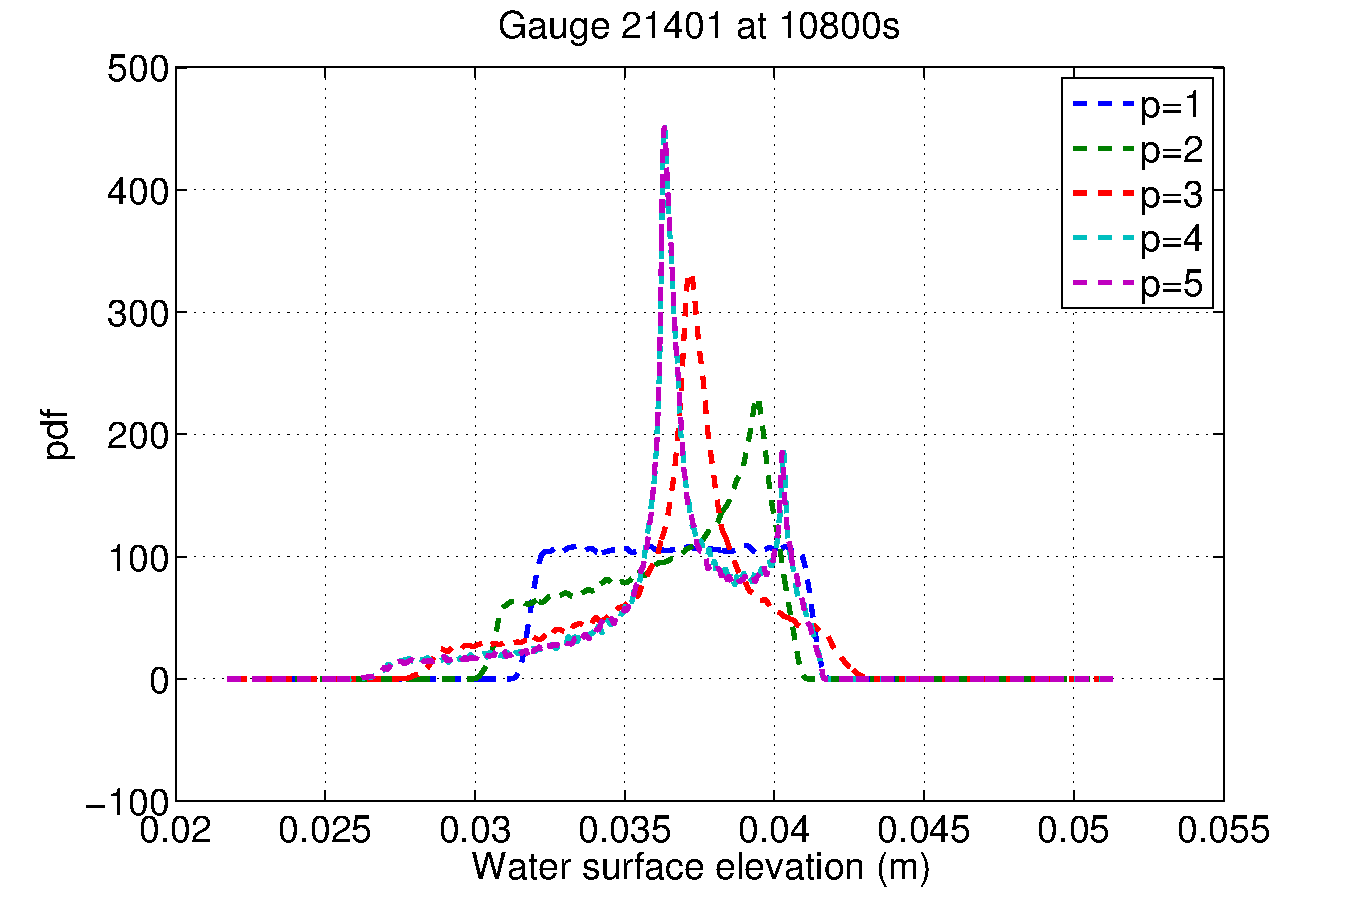
\includegraphics[width=0.5\textwidth]{figures/pdfs1_3.pdf} &
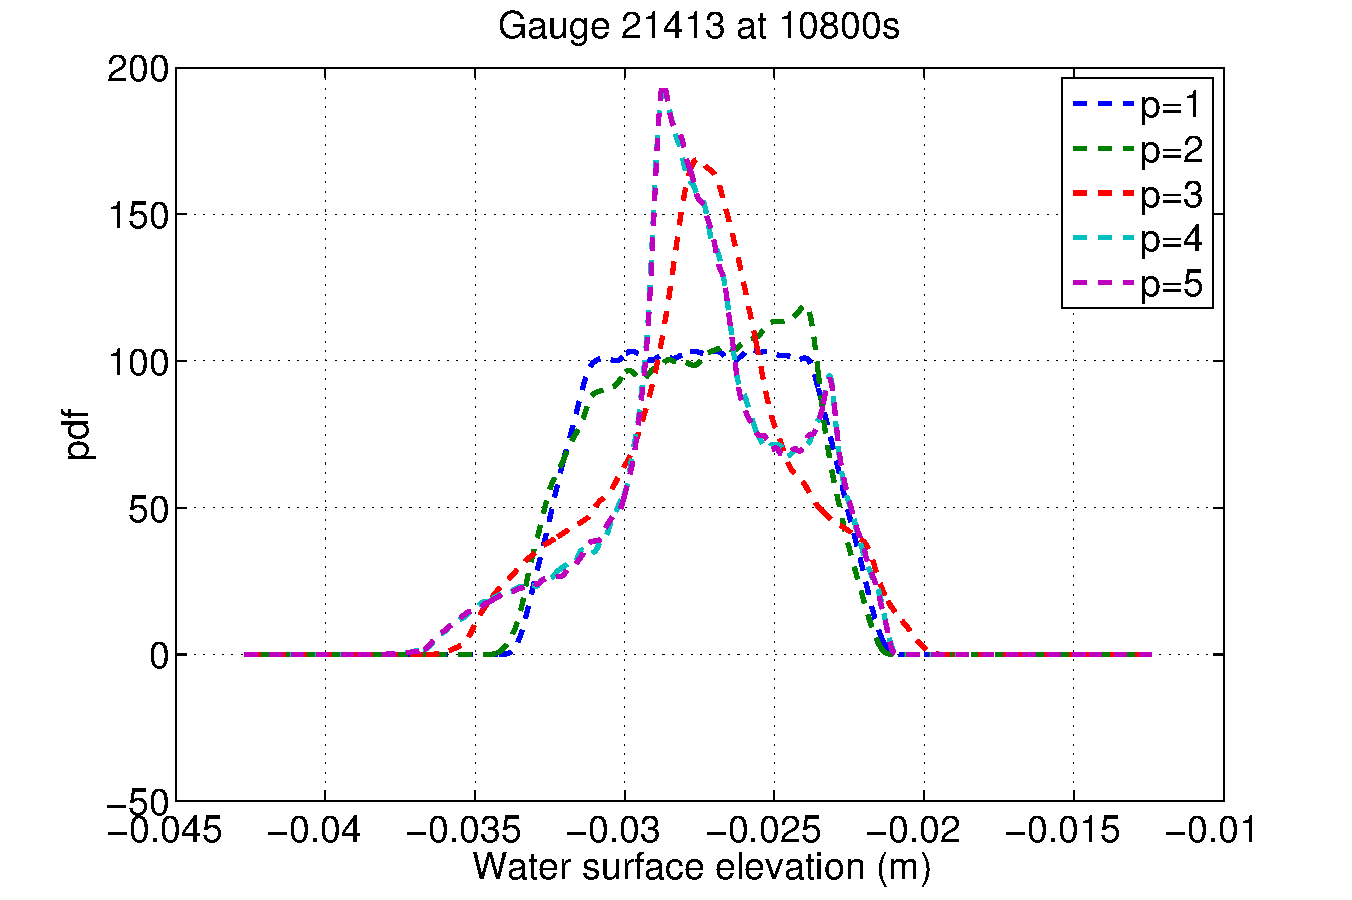
\includegraphics[width=0.5\textwidth]{figures/pdfs2_3.pdf} \\
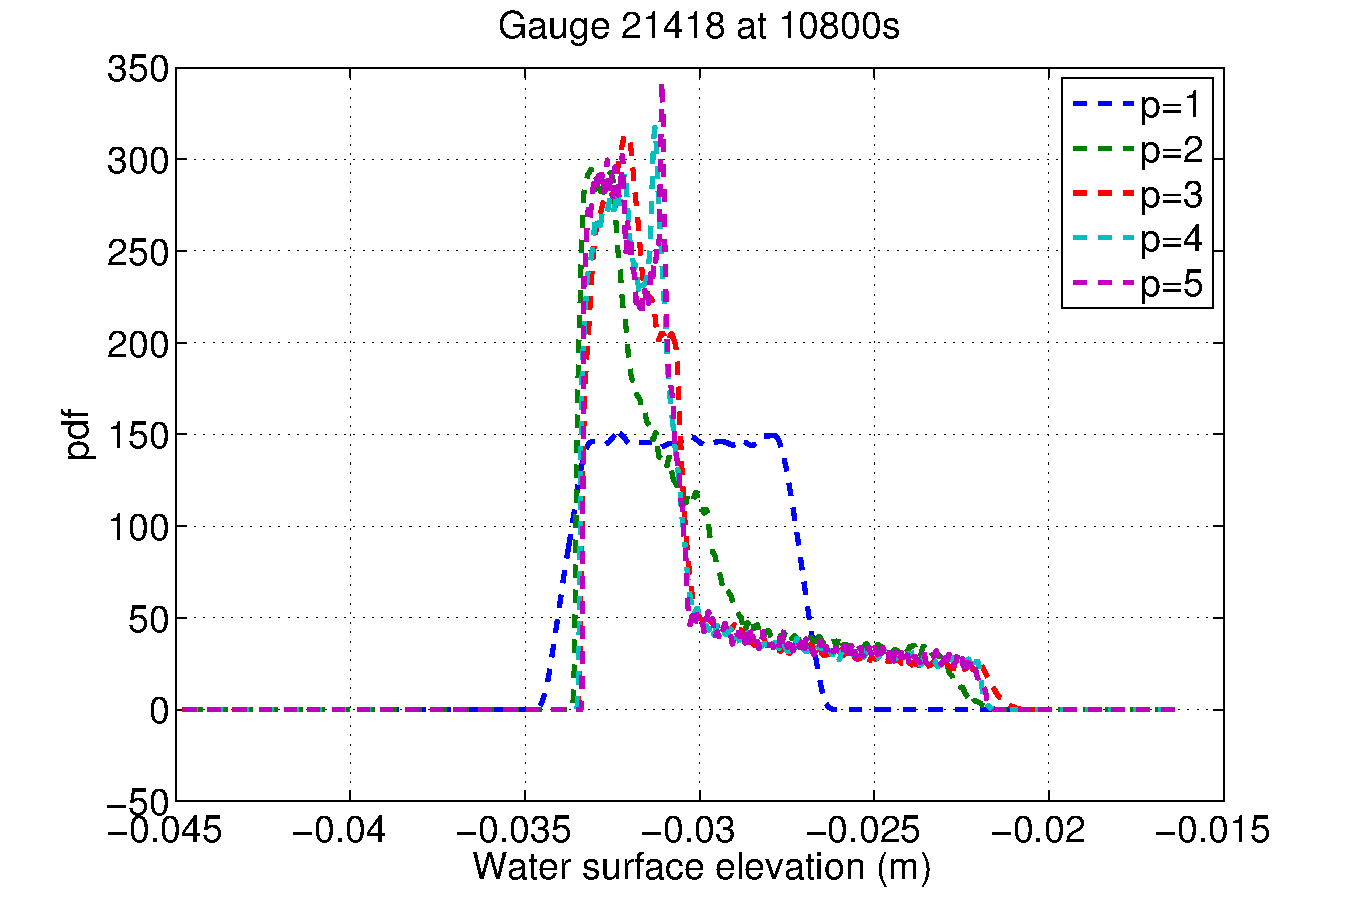
\includegraphics[width=0.5\textwidth]{figures/pdfs3_3.pdf} &
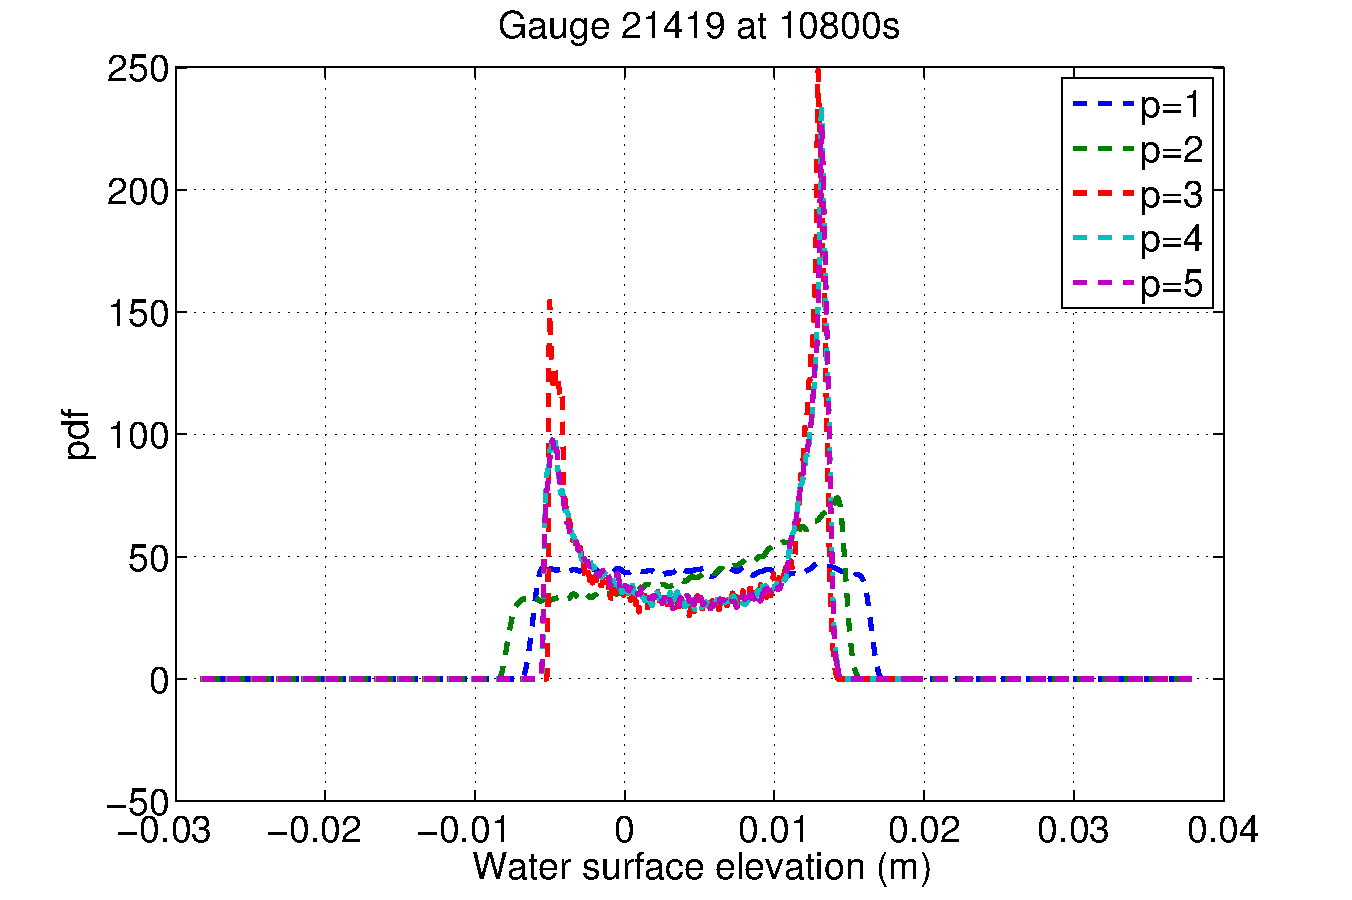
\includegraphics[width=0.5\textwidth]{figures/pdfs4_3.pdf}
\end{tabular}
\caption{pdf of water surface elevation at the different gauge locations at t = 10800 s.}
\label{fig:pdfs3}
\end{figure}
The different curves
correspond to increased order of PC, from 1 to 5; 
The plots indicate that the double peaked distributions are
well-resolved with order  4 but becomes weakly insenstive to further refinement 
as shown with order 5.

The various error metrics presented above 
provide confidence that the PC expansion is a faithful 
model surrogate. 

\clearpage


\subsection{Forward Propagation of Uncertainty}
\label{sec:forward}
The PC expansion created using an ensemble of 125 \geoclaw simulations
is now used as a surrogate to propagate prior input parameter uncertainty 
through the forward model. We here exploit the surrogate 
to study the statistics of the water surface elevation and conduct 
a global sensitivity analysis of the impact of the uncertain input parameters.

\subsubsection{Statistical analysis}
The mean of the QoI and its standard deviation is computed
from the PC coefficients as indicated in Equation~\eqref{eq:mean} and Equation~\eqref{eq:sigma}. 
In Figure~\ref{fig:ave} we plot the evolution of
the calculated PC mean water surface elevation along with two standard deviations
bounds at the four gauges as indicated in each panel.  
Note that we only show the evolution after $t=6000~s$ where the uncertainty is significant,
reflected in a significant standard deviation as seen earlier from the realizations shown 
in Figure~\ref{fig:rlzs}. An interesting observations is that the
standard deviation in water surface elevations vanishes at few times instances
during the tsunami.

These statistics can be used to compare with the 
(DART) buoys observations. Figure~\ref{fig:compare} 
plots the PC mean water surface elevation with the observed 
water surface elevation at the different gauges locations
with error bars indicated at few time instances. 
The plots show a good agreement between the PC simulations and the 
observations at different locations and at different times. 

The same statistical analysis can be performed for the
entire domain in 2D. Figure~\ref{fig:mean2d} (top row) shows
the PC mean water surface elevation for the considered computational
domain at three different times as indicated in the title of each panel.
The standard deviation is also shown in Figure~\ref{fig:mean2d} (bottom row)
at different times. We clearly notice the propagation of the variance
due to the parametric uncertainty with time
and along the tsunami's reflections. 

        
\subsubsection{Sensitivity analysis}
A global sensitivity analysis is next performed to quantity the contribution of each
uncertain parameter to the variance in water surface elevation. To this end, we calculate 
the total sensitivity index using the PC coefficients as shown in Equation~\eqref{eq:T-hard}~\citep{Alexanderian2012,Sudret,Crestaux}. The evolution of the total sensitivity index
of each of the uncertain parameters is shown in Figure~\ref{fig:sens} at the four gauges. 
The Manning's $n$ coefficient at the shore $n_2$ is clearly dominant and contributes
the most to the variance in the water surface elevation compared to the other two 
Manning's $n$ coefficients $n_1$ and $n_3$; this is true for almost the entire simulation time
and at the four gauges. The Manning's $n$ coefficient
in the bottom of ocean $n_{3}$ at gauge number 21419 exhibits small sensitivity index 
during the second hour of simulation and Manning's $n$ coefficient
at the land $n_1$ appears to be an insignificant contributor
to the variance.

In 2D, the sensitivity analysis shows also that $n_2$ is dominant
at the same regions where we observe variance in water surface elevation. This is
indicated from Figure~\ref{fig:sens2d} that shows the total sensitivity index
for $n_1$ (top row) $n_2$ (center row) and $n_3$ (bottom row)
at different times as indicated in each panel.

\subsubsection{Response surface}
In addition to the statistical and sensitivity analysis, the PC surrogate 
can be used to construct a response surface for the uncertain input parameters.
This is achieved by sampling the PC surrogate for different values of the germ $\xxi$ within the prior
range. Since $n_3$ shows insignificant contribution to the 
uncertainty in the model output, we find the impact of $n_2$ and $n_3$ for 
fixed value of $n_1=0.1025$ as illustrated in Figure~\ref{fig:response2}
and Figure~\ref{fig:response3} for different times as indicated. The most striking features are the relatively flat
horizontal contours in the $n_3$ direction suggesting that water surface elevation depends
only mildly on $n_3$ even during peak tsunami events. This is true for gauges 21401, 21413 and 21418. However,
at gauge 21419, its the opposite case where the horizontal contours are in the $n_2 $ direction
and there water surface elevation depends mildly on $n_2$.

\subsection{Inverse Problem} 
\label{sec:inverse}

Before attempting solving the inverse problem,
we need to make sure that the observed data are
comparable to the simulated one. To this end, Figure~\ref{fig:compare}
compares PC mean water surface elevation profiles (with error bars)
with their counterparts from the observed gauge locations.
The plots show a good agreement between the simulations and the 
observations at different locations and at different times. 
The same comparison can be recast as a scatter plot shown in 
Figure~\ref{fig:scatter}. The difference between the observations
and simulations is attributed to the uncertainty in the 
Manning's N coefficient and to the measurement errors to be quantified
in this section.

The surrogate model is exploited in the Bayesian inference of the Manning's 
roughness coefficient.  To this end, an adaptive MCMC method is used to sample 
the posterior distributions \citep{Gareth2009,Haario2001} and consequently 
update the Manning's roughness coefficient distributions in light of the 
observed data. This sampling, demanding tens of thousands of forward simulations, 
would have been prohibitively expensive in the
absence of the surrogate, as the generation of each sample would have required an
independent \geoclaw realization. The surrogate provides a computationally
efficient alternative, and requires only evaluating the PCE for different values 
of the seed $\xxi$. The setup of the Bayesian inference problem,
MCMC chains for the input drag parameters and the corresponding posterior distributions are 
presented and discussed in this section. 


The observed data collected at different locations 
in the likelihood function (Equation~\eqref{eq:likelihood}) to update the input parameters.
MCMCs of $50,000$ iterations are obtained for the Manning roughness coefficients: 
$N_1$,$N_2$ and $N_3$ as well as for the variance $\sigma^2$. Figure \ref{fig:mcmc} 
shows the sample chains for
the input parameters for different iterates of the MCMC algorithms. 
The different panels
shows well-mixed chains for all parameters.
However, all chains span the entire range
of the prior, and so it appears that the observations are not informative 
concerning this uncertain input.  $N_{2}$ chain appears to be concentrated in the lower end of the
parameter range, with values between 0.005 and 0.1.
The chain for the variance is also shown in 
Figure~\ref{fig:mcmc} and appears to be well mixed.





The computed MCMC chains can be readily used to determine the posterior 
distribution; kernel density estimation (KDE) is used for this purpose
~\citep{Parzen1962,Silverman1986}(The first 5000 iterates, associated 
with the burn-in period, are discarded). The resulting posterior pdfs 
of the three Manning's roughness coefficients $N_1,N_2,N_3$ are shown 
in Figure~\ref{fig:pdfs}.  As expected from the chains shown in Figure
~\ref{fig:mcmc}, the posterior pdf of $N_2$, exhibits well-defined peak, 
with a Maximum A Posteriori (MAP) estimate of around 0.011; an extended tail 
towards the higher Manning's roughness coefficient values is also observed.
In contrast, the posterior pdfs of $N_1$ appear to be fairly flat, 
and similar to the uniform prior. This is an indication that 
the observed data were not useful to refine our prior knowledge for $N_1$.
While for $N_3$, we observed a posterior that has a well defined peak
of 0.185 but no clear pdf shape.
The posterior distribution of the variance is also shown in Figure~\ref{fig:mcmc}. 
Taking the square root of the MAP values yields the water surface elevation standard 
deviation, and the latter is a reflection of the mismatch between the model and 
observed data estimated to be 0.145~$m$.


   %MAPS 0.021308543478839   0.011083123405057   0.185744276109897   0.021045124706835




